\section[Тоон гарын үсэг]{Тоон гарын үсгийн стандартын судалгаа}
Хэдийгээр бүх цахим гарын үсэг нь DSS-ийн дүрмийг дагаж мөрдөх ёстой боловч тэдгээр нь бүгд адилхан биш юм. Баримт бичигт гарын үсэг зурахад ашиглаж болох гурван төрлийн тоон гарын үсгийн стандарт байдаг.
\begin{enumerate}
	\item \textbf{Энгийн цахим гарын үсэг (SES)} - Цахим гарын үсгийн хамгийн үндсэн хэлбэр. SES нь баримт бичигт нэмэхэд хурдан бөгөөд хялбар боловч шифрлэлтийн аргаар хамгаалагдаагүй. Өөрөөр хэлбэл, тийм ч аюулгүй биш юм. Үүнд жишээ нь цахим шуудангийн гарын үсэг ордог.
	\item \textbf{Нарийвчилсан цахим гарын үсэг (AES)} - Хэдийгээр хууль ёсны дагуу хүчингүй боловч AES (Advanced Electronic Signature) нь гарын үсэг зурсны дараа баримт бичигт өөрлчлөлт орсон эсэхийг мэдэх боломжтой крифтографыг ашигладаг. Гэсэн хэдий ч хуулийн дагуу хүчингүй хэвээр.
	\item \textbf{Qualified advanced electronic signature (QES)} - Цахим хэлбэрээр гарын үсэг зурах хамгийн найдвартай арга. Тоон гарын үсэг гэж нэрлэгддэг шаардлага хангасан цахим гарын үсэг нь аюулгүй байдлын дээд түвшинг хангахын тулд нийтийн түлхүүрийн дэд бүтэц, тэгш бус криптограф, Two Factor баталгаажуулалтыг ашигладаг. Эдгээрийг ашигласнаар, гарын үсэг нь хууль ёсны дагуу хүчийн төгөлдөр болно.
\end{enumerate}
\section[Ажиллах зарчим]{Тоон гарын үсгийн ажиллах зарчим}
Тоон гарын үсэг нь дижитал мессеж эсвэл баримт бичгийн жинхэнэ эсэхийг шалгах математик аргачлал юм. Энэ нь хос түлхүүр үүсгэх замаар ажилладаг: өргөн тархсан нийтийн түлхүүр, нууцлагдсан хувийн түлхүүр. Гарын үсэг зурахдаа баримт бичгийн өвөрмөц хэшийг үүсгэж, хувийн түлхүүрээр шифрлэж, тоон гарын үсгийг бүрдүүлдэг. Хүлээн авсны дараа хэшийг илгээгчийн нийтийн түлхүүрээр тайлж, хүлээн авсан баримтаас шинэ хэш үүсгэнэ. Хэрэв хоёулаа таарч байвал энэ нь тухайн баримт бичиг нь жинхэнэ бөгөөд ямар нэгэн өөрчлөлт ороогүй гэсэн үг юм.

\begin{figure}
	\centering
	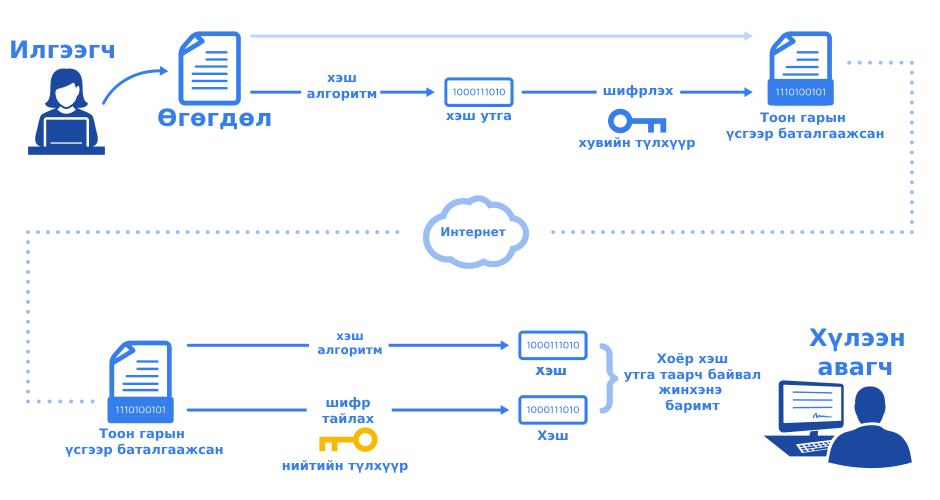
\includegraphics[scale=0.5]{assets/digisigi.png}
	\caption{Тоон гарын үсгийн ажиллах зарчим}
	\label{fig:architecture}
\end{figure}

\section{Адил системийн судалгаа}
\subsubsection{Tridumkey.mn}
Tridimkey нь Монгол улсын бүртгэлийн ерөнхий газраар хүлээн зөвшөөрөгдсөн тоон гарын үсэг олгогч ба байгуулагад зориулж гарын үсэг олгодог нь онцлог санагдсан.
Гэвч сул тал нь энэхүү тоон гарын үсгийн систем нь зөвхөн \textbf{Windows} үйлдлийн систем дээр ажилдаг ба Macos эсвэл Linux үйлдлийн систем ашигладаг хэрэглэгчид ашиглах боломжгүй болж байгаа юм.
\subsubsection{Monpass.mn}
Өөрсдийнх нь танилцуулгад "Таньж баталгаажуулах тоон гарын үсгийн гэрчилгээ: Цахим бизнес, төрийн болон бусад төрөл бүрийн систем, онлайн үйлчилгээнд хандах, бусад цахим гүйлгээ, хэлцэл хийхэд найдвартай таньж баталгаажуулах, захидал харилцааг хөдөлбөргүй баталгаажуулахын тулд тоон гарын үсэг зурах, захидал харилцаа, дамжуулж буй баримт бичгийг шифрлэн дамжуулах, ажилтнууд, хэрэглэгчдийг хялбар таних, бөөний онлайн худалдаа зохион байгуулах гэх мэт зорилгоор ашиглагддаг тоон гарын үсгийн гэрчилгээ – цахим баримт бичиг юм. Энэ гэрчилгээ нь хэрэглэгчийн мэдээлэл, олгосон ГОБ-ын мэдээлэл, хосгүй серийн дугаар болон бусад хосгүй өгөгдлүүд, хүчинтэй хугацаа, тоон гарын үсгийн нийтийн түлхүүр, холбогдох бусад мэдээллийг агуулсан байх бөгөөд Хувь хүмүүс болон байгууллагын төлөөлөгч хэн боловч ашиглаж болно. Захидал, мэдээлэлдээ тоон гарын үсэг зурахдаа өөрийн тоон гарын үсгийн хувийн түлхүүрийг ашиглах ба харин шифрлэн илгээх бол хүлээн авагчийн нийтийн түлхүүрийг ашиглана." гэсэн танилцуулагатай байсан ба гүнзгий судалж үзэхэд мөн л хэрэглэгчийн үйлдлийн систем зөвхөн \textbf{Windows} байж л тоон гарын үсгийн ашиглах боломжтой байсан юм.
\chapter{Системийн судалгаа, зохиомж}
\section{Үүлэн технологийн судалгаа}
Үүлэн технологи буюу үүлэн тооцоолол гэдэг нь өөрийн сервер эсвэл хувийн компьютерын оронд мэдээлэл хадгалах, удирдах, боловсруулах зорилгоор интернэтэд байрлах серверийн сүлжээг ашиглахын хэлж буй нэр томьёо юм.

Үүлэн технологийн хамгийн чухал давуу талуудын нэг нь өртөг багатай байдаг. Үүлэн технологийг ашигласнаар бизнесүүд өөрсдийн мэдээллийн технологийн дэд бүтцээ эзэмших, засвар үйлчилгээ хийх зэрэг урьдчилсан зардал, хүндрэлээс зайлсхийдэг ба зөвхөн ашигласан хэмжээнийхээ зардлыг л төлдөг. Өөр нэг гол давуу тал нь өндөр ачаалал даах уян хатан чанар бөгөөд бизнесүүд тооцоолох хэрэгцээгээ нэмэгдүүлэхийн хэрээр илүү их нөөцийг асар түргэн ашиглах эсвэл тооцоолох хэрэгцээ нь буурах тусам мөн хэрэгцээгээ танах боломжийг шууд олгодог.

Үүлэн технологи нь өгөгдөл сэргээх хадгалах шийдлүүдтэй бөгөөд энэ нь эмзэг мэдээллийг хадгалахад илүү найдвартай сонголт болдог. Хүртээмжтэй байдал нь бизнесүүдийг татдаг үүлэн технологийн бас нэг онцлог юм. Интернэт холболттой бол хэрэглэгчид дэлхийн хаанаас ч өгөгдөл, программдаа хандах боломжтой.

Үүлэн дээр суурилсан тоон гарын үсгийн үйлчилгээ нь хэрэглэгчдэд хүссэн үедээ ямар ч төхөөрөмжөөс баримт бичигт найдвартай гарын үсэг зурах, хадгалах, удирдах боломжийг олгох боломжтой. Энэхүү үйлчилгээ нь баримт бичигт гарын үсэг зурахад заавал биеэр очсон байх шаардлагагүй бөгөөд ингэснээр олон төрлийн үйл явцыг хялбаршуулах боломжтой. Өнөөгийн байдлаар энэ чиглэлд хамгийн томоохон үйлчилгээ үзүүлэгчид нь Amazon Web Services, Google Cloud Platform, Microsoft Azure зэрэг байна.

\pagebreak
\section{Системийн шаардлага}
\subsubsection{Функциональ шаардлагуудыг дараах хүснэгтэд тодорхойлов}
% table
\begin{table}[h]
	\centering
	\caption{Функциональ шаардлага}
	\begin{tabular}{ |p{2cm}|p{13cm}| }
		\hline
		ФШ 100 & Систем нь хэрэглэгчийн тоон гарын үсэг үүсгэх чадвартай байх ёстой. Үүнд хэрэглэгч бүрийн өвөрмөц түлхүүрийн хослолыг бий болгох орно.                                                                             \\ \hline
		ФШ 200 & Систем нь тоон гарын үсгийг баталгаажуулах функцээр хангах ёстой. Энэ нь гарын үсэг зурсан баримт бичгийг хүлээн авч, гарын үсэг зурсан хүний нийтийн түлхүүрийг ашиглан гарын үсгийг баталгаажуулах ёстой.        \\ \hline
		ФШ 300 & Систем нь хэрэглэгчдэд гарын үсэг зурахын тулд янз бүрийн форматтай цахим баримт бичгүүдийг (жишээлбэл, .doc, .pdf, .xls гэх мэт) байршуулахыг зөвшөөрөх ёстой.                                                    \\ \hline
		ФШ 400 & Систем нь хэрэглэгчдийг баримт бичигт гарын үсэг зурах, баталгаажуулахаас өмнө баталгаажуулах ёстой. Үүнийг хэрэглэгчийн нэр/нууц үг, олон хүчин зүйлийн баталгаажуулалт эсвэл бусад аюулгүй аргуудаар хийж болно. \\ \hline
		ФШ 500 & Систем нь баримт бичиг байршуулах, гарын үсэг үүсгэх, гарын үсгийн баталгаажуулалт зэрэг хэрэглэгчдийн хийсэн бүх үйлдлийг бүртгэх ёстой.                                                                          \\ \hline
		ФШ 600 & Систем нь бусад үйлчилгээтэй нэгтгэх API-г өгөх ёстой. Энэ нь бусад программ хангамж эсвэл үйлчилгээнд энэ үйлчилгээний тоон гарын үсгийн чадварыг ашиглах боломжийг олгоно.                                        \\  \hline
		ФШ 700 & Веб нь хэрэглэгч бүртгэх боломжтой байх                                                                                                                                                                            \\ \hline
	\end{tabular}
\end{table}
\pagebreak
\subsubsection{Функциональ бус шаардлагуудыг дараах хүснэгтэд тодорхойлов}
% table
\begin{table}[h!]
	\centering
	\caption{Функциональ бус шаардлага}
	\begin{tabular}{ |p{2cm}|p{13cm}| }
		\hline
		ФБШ 100 & Систем нь GDPR эсвэл HIPAA гэх мэт холбогдох бүх мэдээллийн аюулгүй байдал, нууцлалын дүрэм журмыг дагаж мөрдөх ёстой. Гарын үсэг, баримт бичиг зэрэг бүх өгөгдөл шифрлэгдсэн байх ёстой. \\ \hline
		ФБШ 200 & Систем нь гүйцэтгэлийн бууралтгүйгээр олон тооны хэрэглэгчид болон баримт бичгүүдийг зохицуулах чадвартай байх ёстой.                                                                     \\ \hline
		ФБШ 300 & Үүлэн үйлчилгээ нь хамгийн бага зогсолттой, 24/7 цагийн турш ашиглах боломжтой байх ёстой. Үйлчилгээний түвшний гэрээ (SLA) нь дор хаяж 99.9\% ажиллах хугацааг баталгаажуулах ёстой.     \\ \hline
		ФБШ 400 & Систем нь хүлээн зөвшөөрөгдсөн тодорхой хугацааны дотор гарын үсэг үүсгэх, баталгаажуулах хүсэлтийг хурдан боловсруулах чадвартай байх ёстой.                                             \\ \hline
		ФБШ 500 & Систем нь янз бүрийн техникийн чадвартай хэрэглэгчдэд үүнийг үр дүнтэй ашиглах боломжийг олгодог хэрэглэгчдэд ээлтэй интерфэйстэй байх ёстой.                                             \\ \hline
		ФБШ 600 & Үүлэн үйлчилгээ нь янз бүрийн үйлдлийн систем, хөтөч, төхөөрөмжтэй нийцтэй байх ёстой.                                                                                                    \\  \hline
		ФБШ 700 & Энэ систем нь гамшгийн үед өгөгдөл алдагдахгүй байхын тулд найдвартай нөөцлөх, сэргээх механизмтай байх ёстой.                                                                            \\ \hline
		ФБШ 800 & Систем нь Европ дахь eIDAS эсвэл АНУ-ын ESIGN хууль зэрэг тоон гарын үсгийн хууль тогтоомж, дүрэм журамд нийцсэн байх ёстой.                                                              \\ \hline
	\end{tabular}
\end{table}
\newpage

\section{Use case диаграм}
\begin{figure}[h]
	\centering
	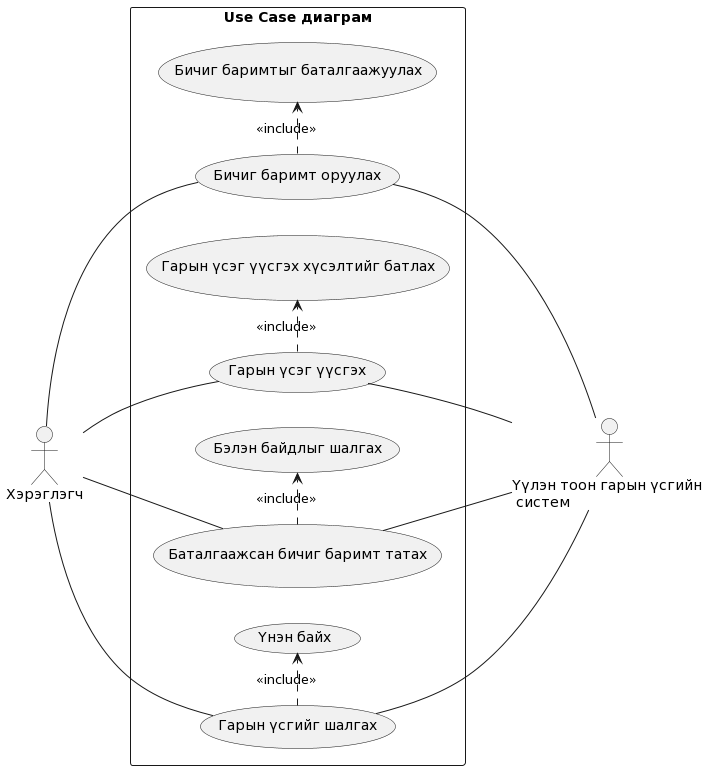
\includegraphics[scale=0.66]{assets/usecase_mn.png}
	\caption{Use case диаграм}
	\label{fig:usecasemn}
\end{figure}
\begin{enumerate}
	\item Хэрэглэгч системийг ашиглан өөрийн бичиг баримтыг зурахын тулд эхлээд эдгээр баримтын систем рүү оруулж өгсөн байх шаардлагатай.
	\item Хэрэглэгч өөрийн гарын үсгийг үүсгэх эсвэл, хүний оролцоогүй системээр автоматаар үүсгүүлэх боломжтой.
	\item Хэрэглэгч баталгаажсан бичиг баримтыг гурав хоногийн дотор татаж авах боломжтой.
\end{enumerate}
\pagebreak
\section{Sequence диаграм}
\begin{figure}[h!]
	\centering
	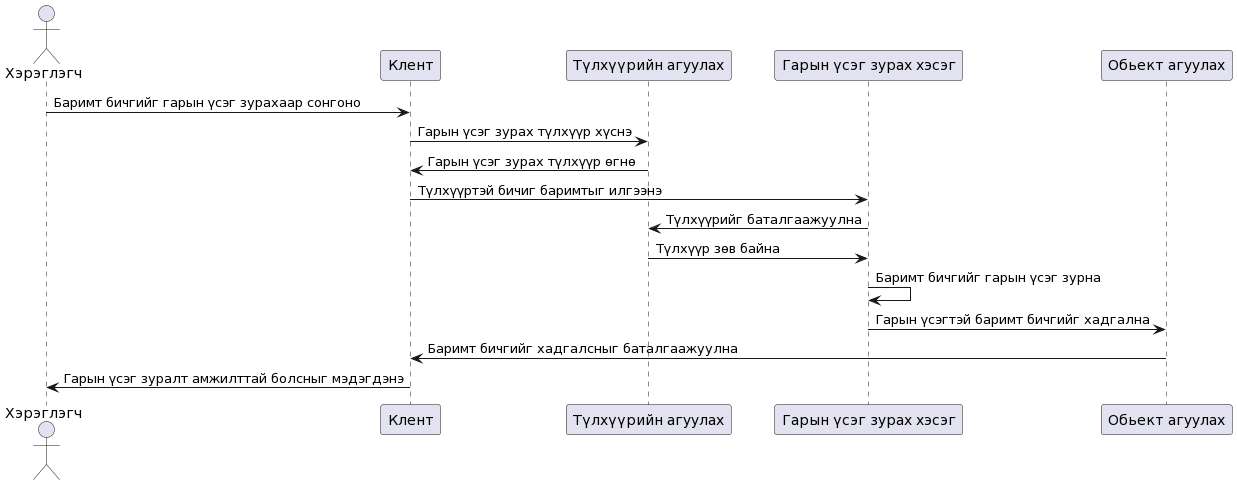
\includegraphics[scale=0.45, angle=90]{assets/sequence2.png}
	\caption{Sequence диаграм}
	\label{fig:usecasemn}
\end{figure}
\newpage
\section{Өгөгдлийн сангийн диаграм}

\begin{figure}[h!]
	\centering
	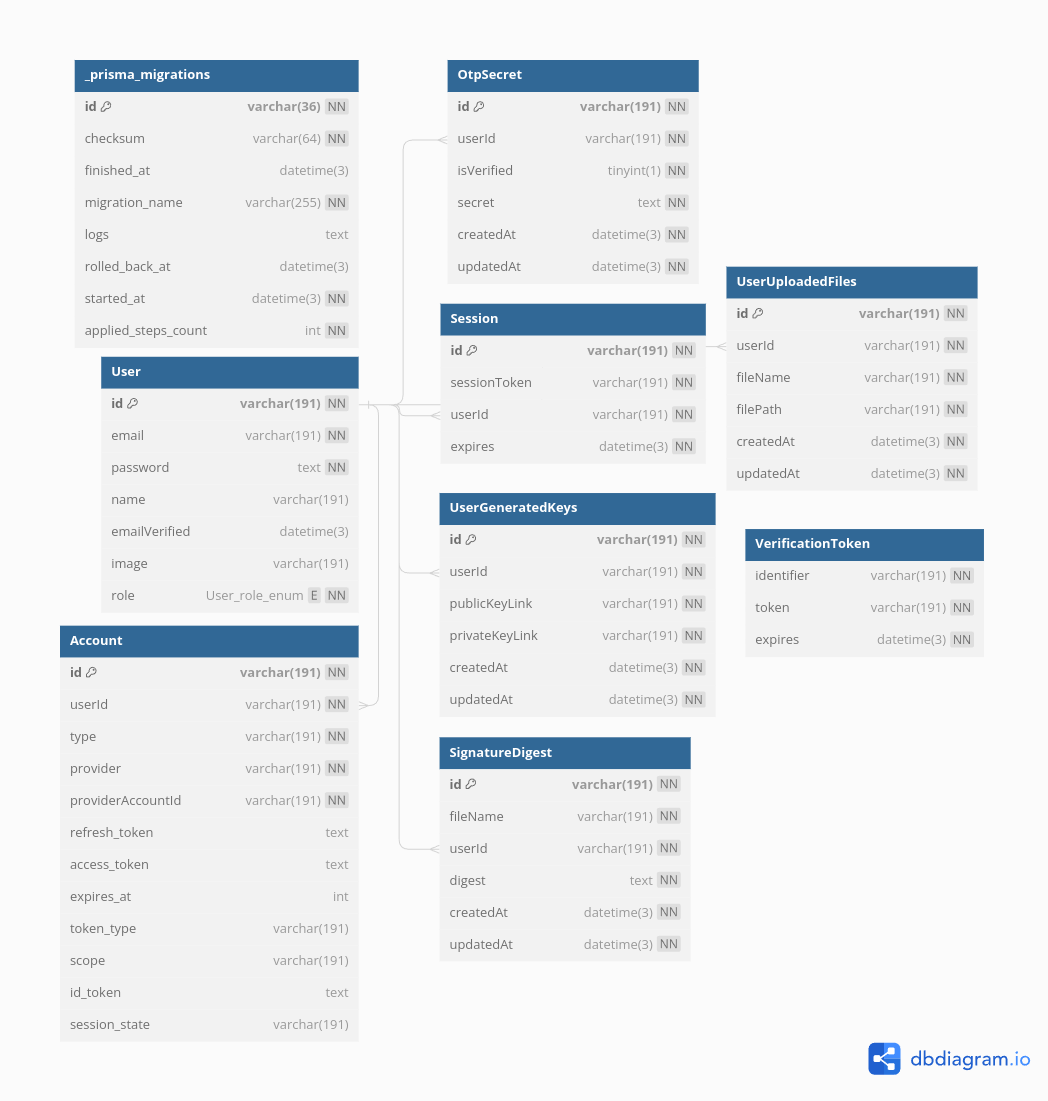
\includegraphics[scale=0.5]{assets/cryptography.png}
	\caption{Датабаз диаграм}
	\label{fig:dbdiagram}
\end{figure}
\break
\newpage
\section{Архитектур}
Энэхүү төслийг ажиллахад илүү хямд зардалтай хүртээмжтэй, ачаалал даах чадварыг нэмэх зорилгоор серверлесс Архитектур сонгосон юм. Фронт-энд хэсэг нь NextJS-н ашигласан тул Сервер талын рендер хийж байгаа ба Бак-энд хэсэг нь тэр чигтээ AWS-н Ламдба функц дээр ажиллах юм. Хэрэглэгчийн серверлүү илгээж байгаа бичиг баримтыг AWS-н Ламдба дээр үүсгэсэн нэг удаагийн холбоосоор хэрэглэгч шууд AWS-руу оруулах юм. Өмнө нь Whatsapp ийм маягаар файл оруулдаг байсан жишээнээс санаа авсан. Статик файлуудыг AWS-н Cloud Front дээр байрлуулсан ба энэ нь дэлхийн өнцөг бүрт байдаг хэрэглэгчид хамгийн ойрхан контент түгээх сүлжээ юм энэ нь хэрэглэгчид илүү хурдан татах боломжийг олгохоос гадна мөн сагхүүгийн хувьд хэмнэлттэй болдог юм. Хэт их хэмжээний хандалт, халдлага зэргээс сэргийлэх зорилгоор AWS-WAF ашиглаж бүх хүсэлтүүд илгээгдэнэ.
\begin{figure}[h!]
	\centering
	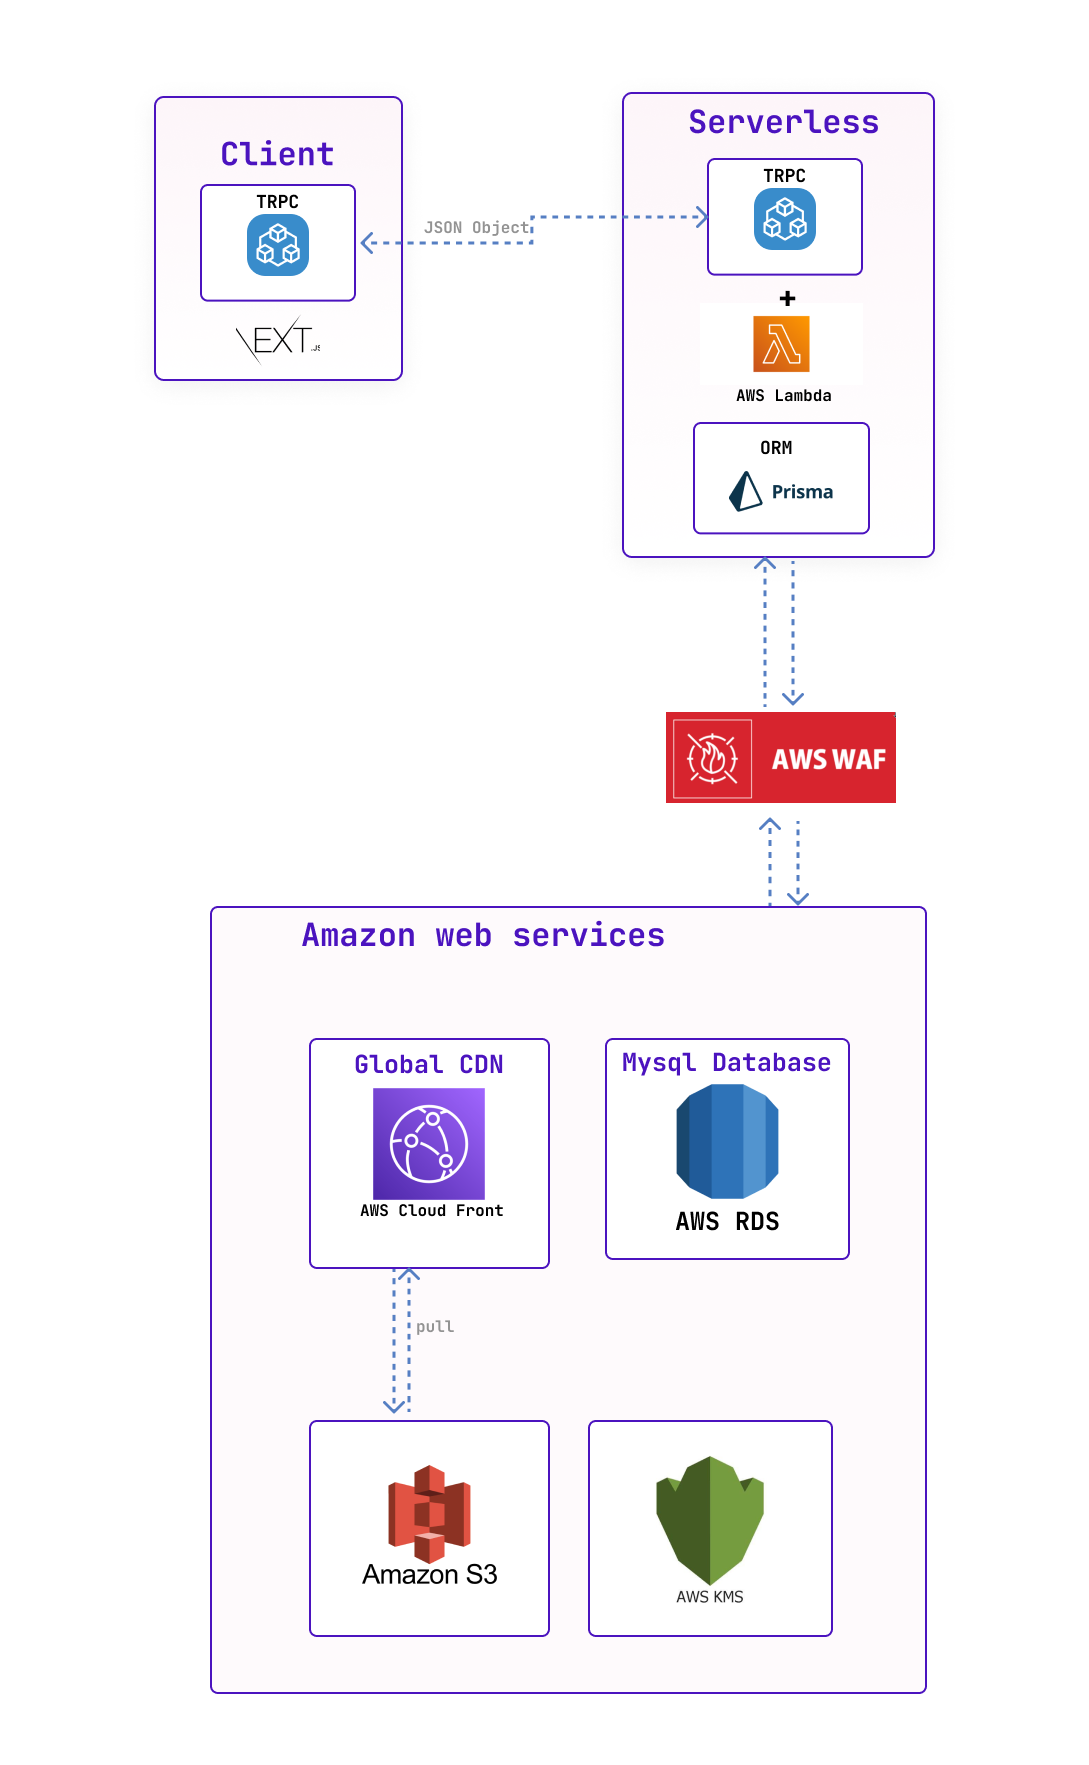
\includegraphics[scale=0.32]{assets/server.png}
	\caption{Архитектур}
	\label{fig:architecture}
\end{figure}
\pagebreak
\newpage
\section[ӨС хүснэгтүүд]{Өгөгдлийн сангийн хүснэгтүүд}

\begin{table}[h]
	\caption{User хүснэгт}
	\begin{tabular}{|l|l|l|p{8cm}|}
	\hline
	№ &  Талбарын нэр & Өгөгдлийн төрөл & Тайлбар \\ \hline
	1 &  id & Varchar & Хэрэглэгчийн дахин давтагдашгүй ID-г хад-
	гална\\ \hline
	2 &  email & Varchar & Хэрэглэгчийн цахим шууданг хадгална\\ \hline
	3 &  password & Varchar & Хэрэглэгчийн нууц үгийг шифрлэж, энэ талбарт хадгална \\ \hline
    4 &  name & Varchar & Хэрэглэгчийн интерфейсээс оруулсан хэрэглэгчийн нэр. Зөвхөн латин үсгийг хадгална. \\ \hline
	5 &  emailVerified & DateTime & Хэрэглэгчийн имэйлийг баталгаажуулсан цагийн тэмдэ \\ \hline
	6 &  image & Varchar & Хэрэглэгчийн байршуулсан зургийн холбоос хадгалагдах бөгөөд зам нь энэ талбарт хадгалагдана \\ \hline
\end{tabular}
\end{table}

\begin{table}[h]
	\caption{Session хүснэгт}
	\begin{tabular}{|l|l|l|p{8cm}|}
	\hline
	№ &  Талбарын нэр & Өгөгдлийн төрөл & Тайлбар \\ \hline
	1 &  id & Varchar & Нэвтрэлтийн түүхийн өвөрмөц ID \\ \hline
	2 &  sessionToken & Varchar & Гуравдагч этгээдийн токен (Github, Google) байна. \\ \hline
	3 &  userId & Varchar & Хэрэглэгчийн өвөрмөц ID \\ \hline
	4 &  expires & DateTime & Дуусах хугацаа \\ \hline
\end{tabular}
\end{table}

\begin{table}[h]
	\caption{UserGeneratedKeys хүснэгт}
	\begin{tabular}{|l|l|l|p{8cm}|}
	\hline
	№ &  Талбарын нэр & Өгөгдлийн төрөл & Тайлбар \\ \hline
	1 &  id & Varchar & Өвөрмөц ID\\ \hline
	2 &  userId & Varchar & Түлхүүрийг үүсгэсэн хэрэглэгчийн ID \\ \hline
	3 &  publicKeyLink & Varchar & Нийтийн түлхүүрийн байршил \\ \hline
	4 &  privateKeyLink & Varchar & Хувийн түлхүүрийн байршил \\ \hline
	5 &  createdAt & DateTime & Үүсгэсэн огноо \\ \hline
	6 &  updatedAt & DateTime & Шинэчилсэн огноо \\ \hline
\end{tabular}
\end{table}
\begin{table}[h]
	\caption{VerificationToken хүснэгт}
	\begin{tabular}{|l|l|l|p{8cm}|}
	\hline
	№ &  Талбарын нэр & Өгөгдлийн төрөл & Тайлбар \\ \hline
	1 &  identifier & Varchar & Токенд зориулсан өвөрмөц ID\\ \hline
	2 &  token & Varchar & Баталгаажуулалтын Токен \\ \hline
	3 &  expires & DateTime & Дуусах хугацаа \\ \hline
\end{tabular}
\end{table}

\begin{table}[h]
	\caption{Account хүснэгт}
	\begin{tabular}{|l|l|l|p{8cm}|}
	\hline
	№ &  Талбарын нэр & Өгөгдлийн төрөл & Тайлбар \\ \hline
	1 &  id & Varchar & Өвөрмрц ID \\ \hline
	2 &  userId & Varchar & Энэ бүртгэлтэй холбоотой хэрэглэгчийн ID \\ \hline
	3 &  type & Varchar & Бүртгэлийн тө \\ \hline
	4 &  provider & Varchar & Аль гуравдагч этгээдийг дамжиж нэвтэрсэн (Github, Google) \\ \hline
	5 &  providerAccountId & Varchar & Хаягийн өвөрмөц ID \\ \hline
    6 &  refresh\_token & Varchar & Шинэ токен үүсгэх нууц үг\\ \hline
    7 &  access\_token & Varchar & Баталгаажуулах токен \\ \hline
    8 &  expires\_at & Int & Дуусах хугацаа\\ \hline
    9 &  token\_type & Varchar & Төрөл \\ \hline
    10 &  scope & Varchar & Нэвтрэлтийн эрх \\ \hline
    11 &  id\_token & Varchar & Өвөрмөц ID \\ \hline
    12 &  session\_state & Varchar & Одоо нэвтрэлттэй байгаа эсэх\\ \hline
\end{tabular}
\end{table}

\begin{table}[h]
	\caption{UserUploadedFiles хүснэгт}
	\begin{tabular}{|l|l|l|p{8cm}|}
	\hline
	№ &  Талбарын нэр & Өгөгдлийн төрөл & Тайлбар \\ \hline
	1 &  id & Varchar & Хэрэгдэгчийн оруулсан файлын өвөрмөц ID\\ \hline
	2 &  userId & Varchar & Файлыг байршуулсан хэрэглэгчийн ID \\ \hline
	3 &  fileName & Varchar & Файлын нэр\\ \hline
	4 &  filePath & Varchar & Файл хадгалагдаж буй зам \\ \hline
	5 &  createdAt & DateTime & Файлыг байршуулсан цаг \\ \hline
	6 &  updatedAt & DateTime & Файлын мэдээлэл хамгийн сүүлд шинэчлэгдсэн цаг \\ \hline
\end{tabular}
\end{table}

\begin{table}[h]
	\caption{OtpSecret хүснэгт}
	\begin{tabular}{|l|l|l|p{8cm}|}
	\hline
	№ &  Талбарын нэр & Өгөгдлийн төрөл & Тайлбар \\ \hline
	1 &  id & Varchar & Нэг удаагийн нууц үг үүсгэх түлхүүрийн ID\\ \hline
	2 &  userId & Varchar & Холбоотой хэрэглэгчийн ID \\ \hline
	3 &  isVerified & Boolean & OTP нь баталгаажсан эсэх \\ \hline
	4 &  secret & Text & Нэг удаагийн нууц үгийн баталгаажуулалтад ашигласан нууц \\ \hline
	5 &  createdAt & DateTime & OTP үүсгэсэн цаг\\ \hline
	6 &  updatedAt & DateTime & Хамгийн сүүлд шинэчилсэн цаг\\ \hline
\end{tabular}
\end{table}

\begin{table}[h]
	\caption{SignatureDigest хүснэгт}
	\begin{tabular}{|l|l|l|p{8cm}|}
	\hline
	№ &  Талбарын нэр & Өгөгдлийн төрөл & Тайлбар \\ \hline
	1 &  id & Varchar & Нууц үгийн хайшийн ID\\ \hline
	2 &  fileName & Varchar & Холбогдсон файлын нэр \\ \hline
	3 &  userId & Varchar & Харгалзах хэрэглэгчийн ID\\ \hline
	4 &  digest & Text & Хайшын утга \\ \hline
	5 &  createdAt & DateTime & Үүсгэсэн огноо \\ \hline
	6 &  updatedAt & DateTime & Шинэчилсэн огноо \\ \hline
\end{tabular}
\end{table}

\pagebreak
\newpage

